\chapter{Metodologie di Analisi}
\label{ch:capitolo3}

\begin{flushleft}
    
Nel corso di questo capitolo sarà presentata una panoramica delle metodologie di analisi e delle pipeline (figura \ref{fig:pipeline}) per la costruzione dei modelli, i risultati di tali analisi saranno poi disponibili nel capitolo successivo.
È importante sottolineare che, a causa delle policy aziendali, non sarà possibile fornire il codice scritto.

Segue un elenco delle tecnologie,librerie e degli strumenti utilizzati durante lo stage:
\begin{itemize}
    \item \textbf{Python 3.10}: Tutto il codice da me scritto, dalla creazione dei modelli, alle analisi sui dati è stato in tale linguaggio di programmazione.
    Le librerie utilizzate sono state le seguenti:
    \begin{itemize}
    \item statistics
    \item interpret
    \item dice ml
    \item pandas
    \item numpy
    \item scipy
    \item imblearn
    \item matplotlib
    \item sklearn
    \item seaborn
    \item json
    \item configparser
    \item ydata\_profiling
    \item webbrowser
\end{itemize}
    \item \textbf{Google Colab}: Strumento usato per eseguire i test in parallelo
    \item \textbf{Notion}: Strumento usato per salvare, impostare ed elaborare i risultati dei test
    \item \textbf{Jupiter Notebook}: Strumento usato per creare un ambiente di lavoro più pulito e sequenziale

\end{itemize}

\begin{figure}[H]
    \centering
    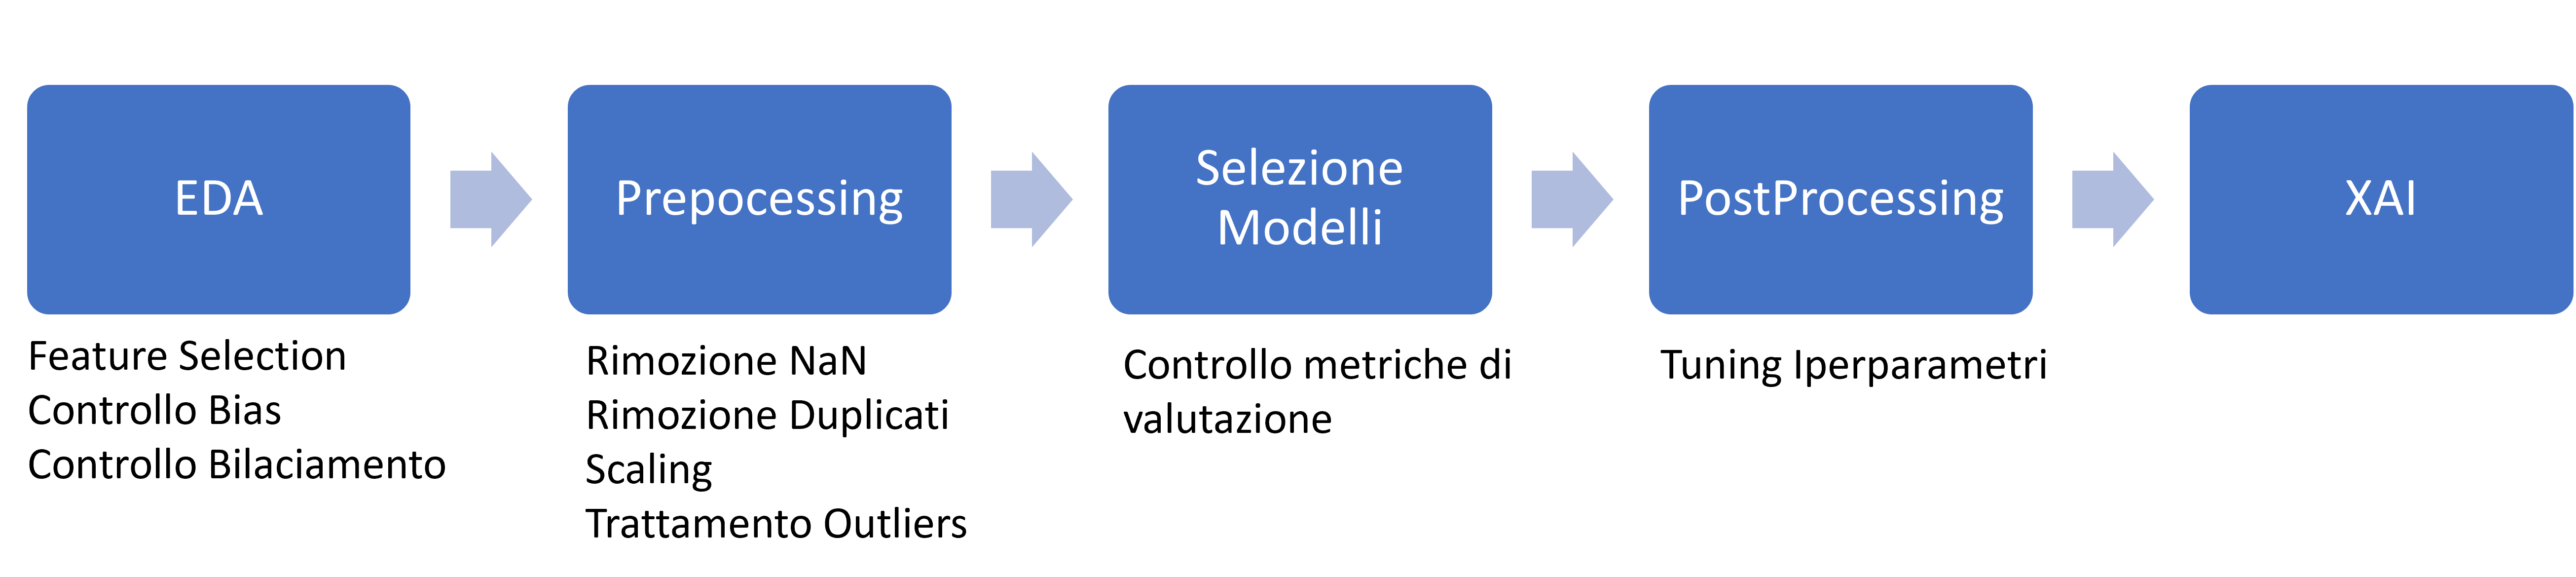
\includegraphics[width=1\linewidth]{TemplateTesi//immagini/pipeline.png}
    \caption{Pipeline di Lavoro Generale attuata}
    \label{fig:pipeline}
\end{figure}

\section{Esplorazione Iniziale dei Dati (EDA)}
L'analisi esplorativa dei dati è un processo fondamentale per comprendere la struttura, le caratteristiche e le relazioni presenti all'interno di un dataset. 
Il primo passo è stato quello di condurre una ricerca per capire le caratteristiche dei i dati clinici relativi alla problematica per la quale si doveva trovare una soluzione. L'obiettivo era identificare i parametri, o feature, più significative per la classificazione del problema precedentemente illustrato.

Durante questa fase, sono stati selezionati i dataset più promettenti dalla piattaforma "Kaggle", effettuando una scrematura che teneva conto della tipologia delle feature presenti, dell'affidabilità delle fonti, della provenienza geografica dei dati e del parametro interno di Kaggle chiamato "Usability". Questo parametro tiene in considerazione le seguenti caratteristiche del dataset: completezza, credibilità e compatibilità.
I dataset analizzati sono strutturati in modo tale che le colonne rappresentino le diverse feature, mentre le righe corrispondono a singoli pazienti, contenendo così i record delle relative feature.
Tali dataset sono visualizzabili in figura~\ref{fig:datasets}.

\begin{figure}[H]
    \centering
    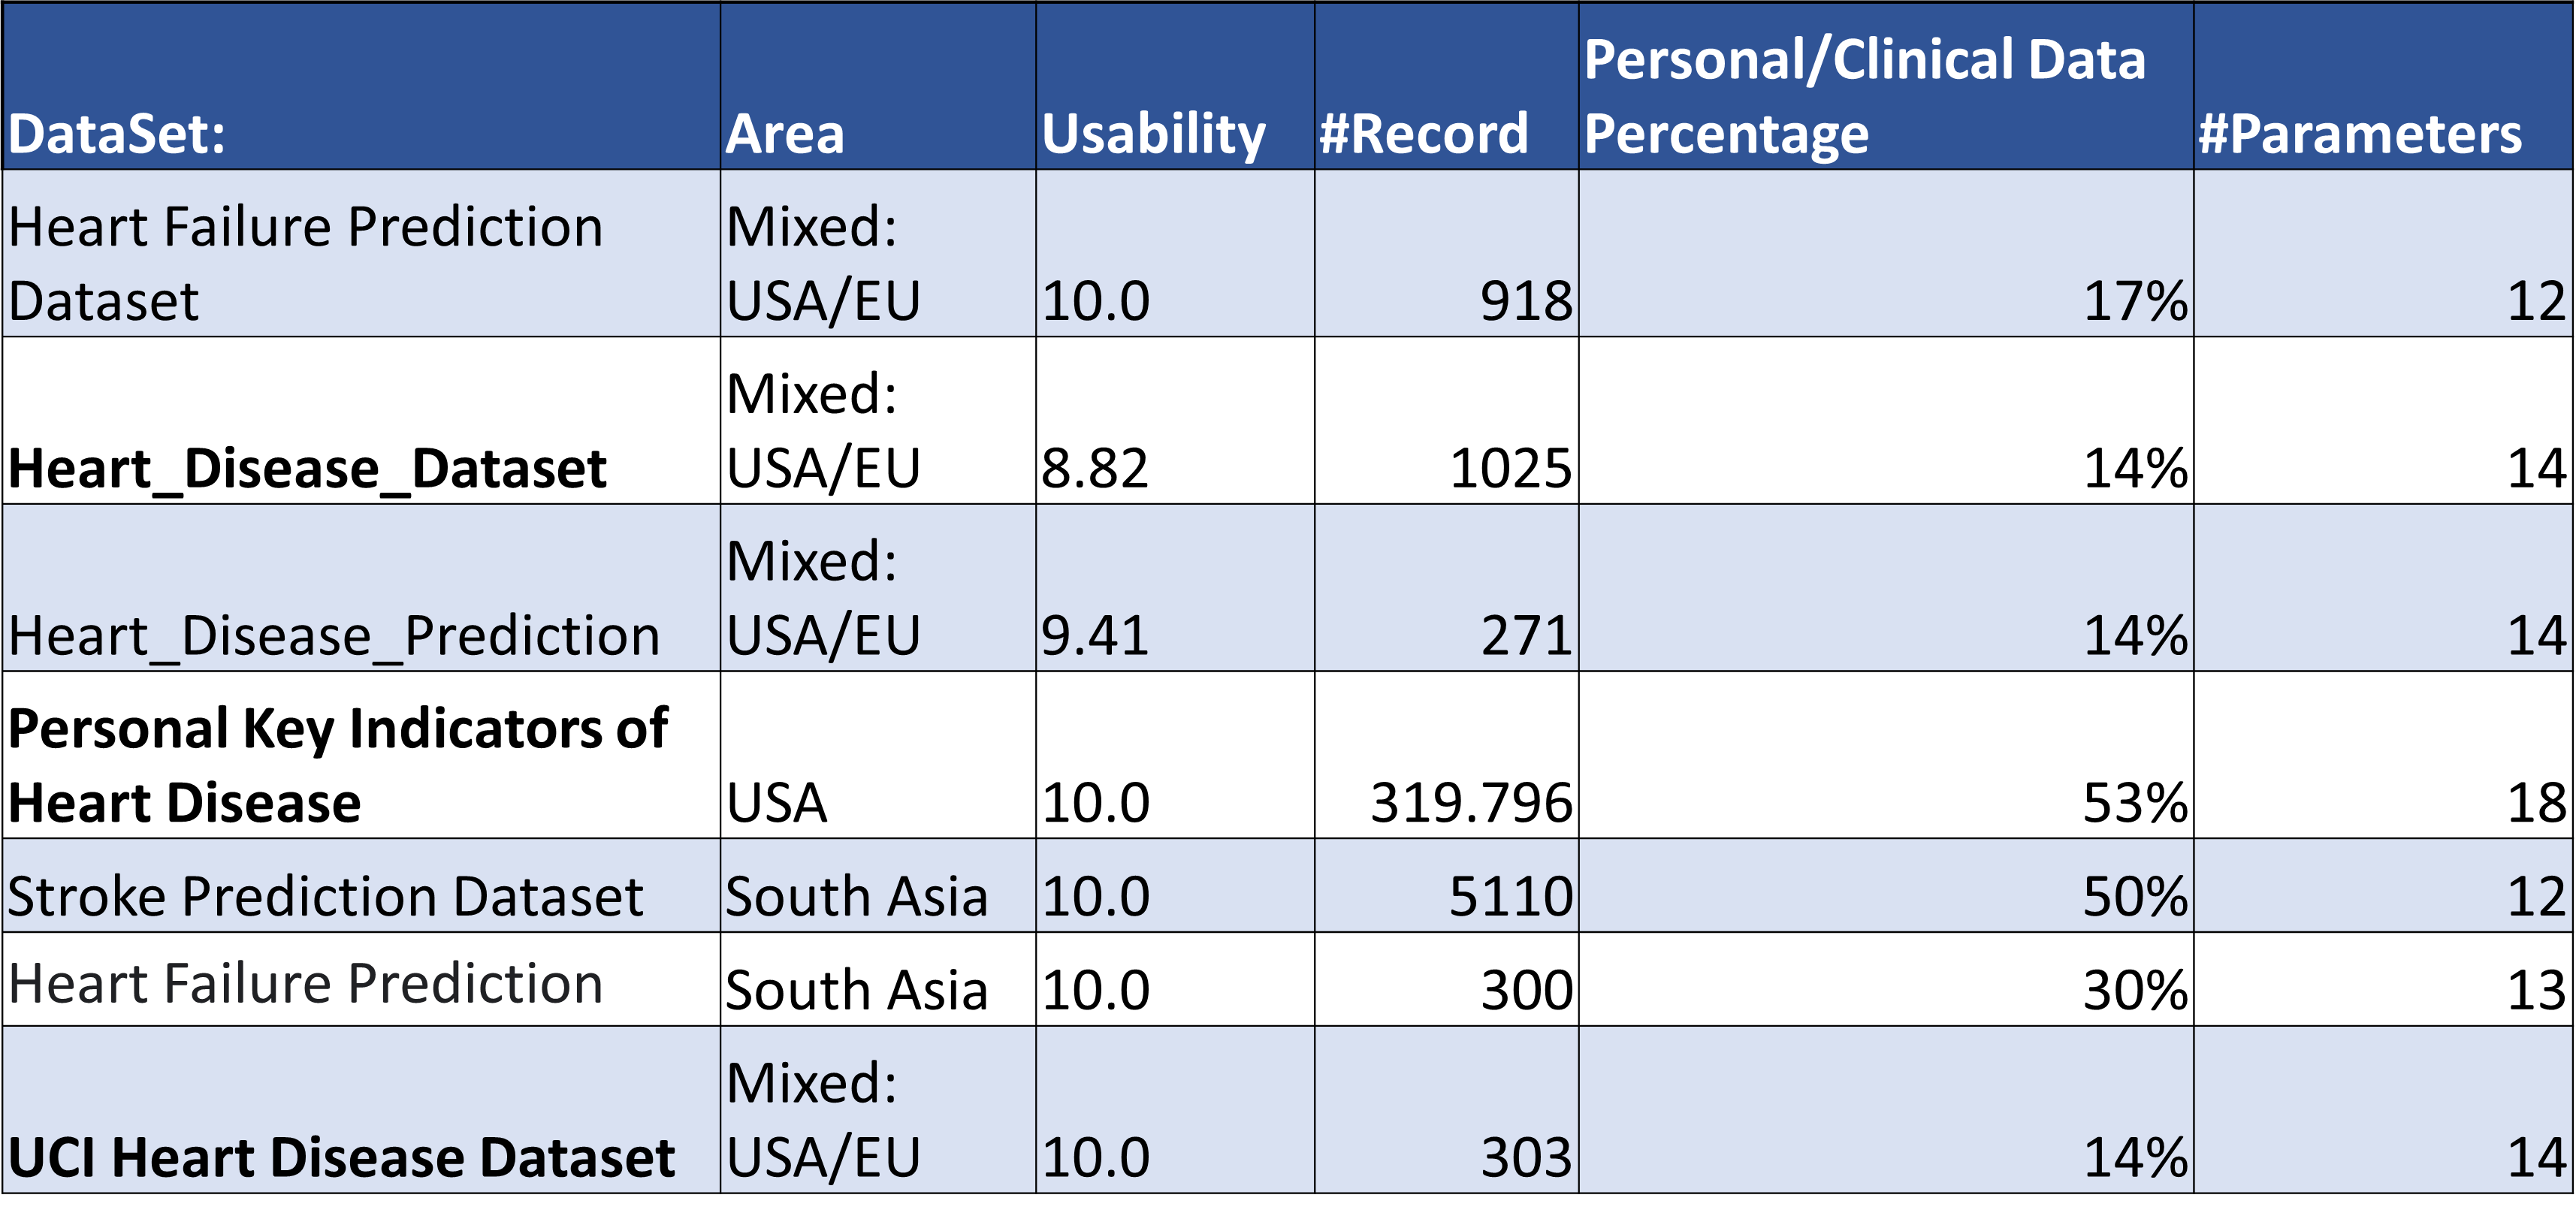
\includegraphics[width=1\linewidth]{TemplateTesi//immagini/datasetsgrassetto.png}
    \caption{I DataSet Selezionati}
    \label{fig:datasets}
\end{figure}

Una volta che i dataset sono stati selezionati, sono state condotte analisi su ciascuno di essi al fine di individuare le feature più significative per la classificazione.
Tra le analisi più importanti effettuate rientrano:
\begin{itemize}
    \item Calcolo dei coefficienti di correlazione tra le feature e tra feature e target
    \item Calcolo delle distribuzioni di probabilità delle feature
    \item Calcolo del MI score 
    \item Analisi qualitativa delle distribuzioni con i clinici
\end{itemize}
Dato il numero considerevole di dataset presi in esame,si riporteranno nella tesi i risultati di tre di essi, che sono coerenti con quelli relativi agli altri dataset: "Heart Disease Dataset (HDD)", "UCI Heart Disease (UCI)" e "Personal Key Indicator of Heart Disease"(PKI).
Su questi tre dataset sono poi state applicate le tecniche di ML studiate.

Il primo e il secondo dataset presentano un'alta percentuale di feature di tipo clinico, mentre il terzo dataset contiene un buon numero di feature che saranno denominati "Personali". Questi dati non derivano da strumentazioni mediche, ma sono accessibili tramite un semplice sondaggio. L'inclusione di questi dati personali è di fondamentale importanza poiché semplifica e velocizza l'acquisizione delle informazioni, evitando di gravare sulle risorse della struttura ospedaliera o richiedere tempo al personale medico.

Prima di presentare le analisi effettuate segue una breve spiegazione delle feature dei dataset menzionati.

\subsubsection{Heart Disease Dataset (HDD)}
%TODO DIRE PROVENIENZA DATI E INTRODURRE LE FEATURES MEGLIO
Il dataset HDD è composto principalmente da features cliniche e i dati provengono dal repository "UCI Machine Learning Repository".
Presenta le seguenti feature:
\begin{itemize}
  \item Age: Età
  \item Sex: Sesso
  \item cp: Tipologia di dolore al petto
  \item trestbps: Pressione Sanguigna a Riposo
  \item chol:colesterolo sierico in mg/d
  \item fbs: glicemia a digiuno
  \item restecg: ECG a riposo
  \item thalach : Massimi Battiti cardiaci raggiunti
  \item exang : angina indotta dall'esercizio fisico
  \item oldpeak:ST depression, ovvero ad un'alterazione del tratto ST dell'elettrocardiogramma di superficie
  \item slope: ST slope
  \item ca: numero di vasi colorati con fluoroscopia
  \end{itemize}

\subsubsection{Personal Key Indicator Of Heart Disease (PKI)}


PKI è un dataset recentemente costruito attraverso l'utilizzo di sondaggi. 
PKI presenta un numero significativamente alto di record, questi sono formati per metà da features di tipo personale.
Seguono le features con le relative domande poste dal sondaggio:


\begin{itemize}
\item HeartDisease: Soggetti che hanno segnalato di aver avuto malattia coronarica o infarto miocardico 
\item BMI: Indice di massa corporea (BMI)
\item Smoking: Hai mai fumato almeno 100 sigarette durante tutta la tua vita? 
\item AlcoholDrinking: Sei un consumatore eccessivo di alcol ? (uomini adulti che assumono più di 14 bevande alcoliche a settimana e donne adulte che assumono più di 7 bevande alcoliche a settimana)
\item Stroke: Ti è mai stato detto che hai avuto un infarto?
\item PhysicalHealth: Pensando alla tua salute fisica, che include malattie e lesioni fisiche, per quanti giorni nei 30 passati la tua salute fisica non è stata buona? 
\item MentalHealth: Pensando alla tua salute mentale, per quanti giorni nei 30 passati la tua salute mentale non è stata buona? 
\item DiffWalking: Hai seri problemi a camminare o salire le scale?
\item Sex: Sei maschio o femmina?
\item AgeCategory: Categoria di età su quattordici livelli
\item Etnia: A che etnia appartieni ?
\item Diabetic : Ti è mai stato detto che hai il diabete?
\item PhysicalActivity: Adulti che hanno dichiarato di fare attività fisica o esercizio durante gli ultimi 30 giorni, al di fuori del lavoro abituale
\item GenHealth: Come descriveresti in generale la tua salute ?
\item SleepTime: In media, quante ore di sonno dormi in un periodo di 24 ore?
\item Asthma: Ti è mai stato detto che hai l'asma?
\item KidneyDisease: Escludendo calcoli renali, infezioni alla vescica o incontinenza, ti è mai stato detto che hai una malattia renale?
\item SkinCancer:Ti è mai stato detto che hai avuto il cancro della pelle?
\end{itemize}

\subsubsection{UCI Heart Disease Dataset (UCI)}


Durante la fase finale del mio stage ho effettuato un'analisi del seguente dataset aggiungendolo al set di dataset esistenti. La decisione di includere questo dataset è stata motivata dalla mia volontà di creare un modello che fosse il più indipendente possibile da complessità aggiuntive. Pertanto, ho cercato di limitare l'applicazione di tecniche sullo stesso, escludendo tecniche di outlier detection e feature selection.

Il dataset in questione è una versione rielaborata del dataset originale noto come "UCI Heart Disease", da cui HDD e gli altri dataset clinici prendono forma. UCI si basa su dati provenienti da quattro database situati in Ungheria, Svizzera, Cleaveland e Long Beach.
Il dataset HDD, a differenza di quest'ultimo, presenta un numero di record superiore rispetto al dataset originale.

Le feature del suddetto dataset e le considerazioni sulle caratteristiche di queste ultime sono identiche a quelle presenti in HDD, quindi non verranno nuovamente menzionate.



\section{Preprocessing dei dati}

In questa sezione,sono illustrate le tecniche di preprocessing che \textbf{sono state applicate ad ogni dataset preso in esame}.
Come spiegato nel capitolo 2, il preprocessing dei dati è una fase cruciale nella preparazione di un dataset per l'applicazione degli algoritmi di ML.
Le tecniche di preprocessing che sono state adottate includono la conversione dei valori nominali in valori numerici, l'eliminazione delle righe con dati mancanti o NaN, l'eliminazione dei duplicati e la normalizzazione dei dati.

\subsection{Conversione dei valori nominali in valori numerici} 
Nei dataset originali, alcune variabili contenevano valori nominali. Per poter utilizzare queste variabili nell'analisi, è stato necessario convertire i valori nominali in valori numerici. Questa conversione è stata effettuata assegnando un valore numerico univoco a ciascuna categoria presente nella variabile nominale. Ad esempio, nel dataset 'PKI' alla variabile 'Sex'i cui valori precedenti erano "Male" e "Female" sono stati assegnati rispettivamente "1" e "0"

\subsection{Eliminazione delle righe con dati mancanti o NaN}
Durante l'analisi dei dataset, è stata rilevata a volte la presenza di alcune righe con dati mancanti o NaN. Sebbene il numero di valori mancanti era relativamente basso si è deciso di eliminare interamente le righe che presentavano dati mancanti o NaN, poiché tale eliminazione non avrebbe compromesso significativamente la rappresentatività dei dati.

\subsection{Eliminazione dei duplicati}
Al fine di evitare la duplicazione dei dati, è stata eseguita un'operazione di rimozione dei duplicati. I duplicati sono stati individuati confrontando l'intera riga di ciascun record con le altre righe del dataset attraverso l'utilizzo di funzioni di libreria.
Se due righe presentavano gli stessi valori in tutte le colonne, tranne l'identificatore univoco del record, una delle righe duplicate è stata eliminata.

\subsection{Normalizzazione dei dati}
La normalizzazione dei dati è una pratica comune nel preprocessing dei dati, che mira a rendere le diverse variabili comparabili nello stesso intervallo di valori. Durante l'analisi, sono state esplorate diverse tecniche di normalizzazione, tra cui MinMax Scaling, Standard Scaler e Robust Scaling. Tutte e tre le tecniche hanno prodotto risultati comparabili, ma alla luce della loro semplicità e della facilità di interpretazione dei risultati, è stata scelta la tecnica di Standard Scaling per la normalizzazione dei dati.

\subsection{Eliminazione degli outlier}
Come specificato nel Capitolo 2, la presenza di outlier può influenzare negativamente i risultati dell'analisi e alterare le conclusioni ottenute. 
Pertanto, è importante identificare e trattare gli outlier in modo appropriato.
Per fare ciò è stata applicata la tecnica di identificazione degli outlier dello Z-score (Figura \ref{fig:zscore}) con valore soglia variabile (generalmente  intorno a 3.5).
Una volta identificati gli outlier è stata rimossa la riga dal dataset che lo rappresentava.

\section{Scelta dei Modelli e Iperparametri}
 Una volta completate le fasi di analisi esplorativa dei dati e preprocessing, si è passato alla fase di addestramento dei modelli.

La scelta del modello è una decisione fondamentale per la creazione di un tool di AI, poiché diversi algoritmi di ML possono adattarsi in modo ottimale a diverse tipologie di dati e problemi specifici. Pertanto, ho valutato  quattro modelli di ML diversi.

\begin{itemize}
    \item SVM
    \item XGB
    \item RF
    \item ADA
\end{itemize}

Durante il processo di selezione del modello, ho considerato diverse metriche di valutazione, tra cui l'accuracy, la precision, la recall, al fine di identificare il modello che avesse le migliori prestazioni nel contesto del mio problema di classificazione.

Dopo aver selezionato il modello, ho valutato le metriche ottenute tramite la cross-validation, utilizzando il 70\% dei dati per l'addestramento e il restante 30\% per i test. Successivamente, ho proceduto con la selezione degli iperparametri.



\subsection{Bilanciamento dei Dataset}

Uno sbilanciamento dei dati, come discusso nel capitolo precedente, può influire negativamente sulle prestazioni del modello, in quanto può verificarsi una predizione sbilanciata o una maggiore sensibilità verso la classe dominante.

Considerando le caratteristiche dei dataset su cui ho lavorato ho valutato l'applicazione delle tecniche di bilanciamento denotate in precedenza, ovvero quelle di undersampling e oversampling.

\subsection{Selezione dei Modelli} 

Dopo aver valutato i quattro modelli di ML, è stata effettuata una comparazione dei  risultati della cross validation. Sulla base delle metriche di valutazione e delle esigenze specifiche del nostro problema (SVM ad esempio è stato scartato poichè i tempi di addestramento erano eccessivamente lunghi, a volte superiori alle 24H per PKI), sono stati selezionati i due modelli che hanno mostrato le migliori prestazioni complessive:  il Modello XGB e il Modello RF .

Tra i due modelli selezionati è stato condotto un ulteriore confronto per determinare il modello più performante. Dopo un'analisi dei risultati, è stato decretato che il Modello RF era il modello più efficace e adatto alle mie esigenze.


\subsection{Ricerca degli iperparametri}
Una volta trovato il modello più performante,l'ultimo passo per migliorare lo score delle metriche è stata la ricerca degli iperparametri, per fare ciò ho adottato un approccio ibrido che combina la random search e la grid search.

Per iniziare, ho utilizzato la random search come tecnica per l'analisi iniziale degli iperparametri. La random search ha consentito l'esplorazione di un'ampia gamma di combinazioni di iperparametri selezionati in maniera casuale. Questo mi ha permesso di ottenere una visione generale delle prestazioni dei modelli con diverse configurazioni di iperparametri, consentendomi di individuare alcune combinazioni più promettenti.

Una volta identificate le combinazioni più promettenti grazie alla random search, ho approfondito la ricerca in un intorno di quegli iperparametri utilizzando la grid search. 

Come spiegato precedentemente la grid search è una tecnica di ricerca esaustiva che valuta tutte le possibili combinazioni di iperparametri specificate in un insieme predefinito, sotto forma di griglia.

Una volta creata la griglia di valori, la grid search ha quindi valutato tutte le possibili combinazioni di questi valori per trovare il set di iperparametri ottimale.

L'approccio ibrido ha dimostrato di essere un metodo efficace per trovare iperparametri ottimali in modo estremamente efficiente. 
Ha permesso di bilanciare la copertura di un'ampia gamma di combinazioni con una ricerca più dettagliata nell'intorno di quelle combinazioni più promettenti.

\section{XAI}
Una volta completata la fase di costruzione dei modelli,
ho messo in pratica tecniche di XAI per fornire spiegazioni dei risultati ottenuti dai miei modelli. In particolare, ho utilizzato sia il metodo LIME che le Counterfactual Explanations, che mi hanno permesso di analizzare il mio problema e le soluzioni sviluppate da un'altra prospettiva. Questo approccio ha arricchito la comprensione dei modelli e ha fornito una maggiore trasparenza riguardo alle ragioni alla base delle previsioni effettuate,di fondamentale importanza nell'ambito clinico.

\subsection{LIME}
L'interpretabilità dei modelli riveste un ruolo fondamentale in ambito clinico, la spiegazione fornita da LIME mi ha aiutato a a identificare le caratteristiche più rilevanti per una determinata predizione e fornire indicazioni su quali aspetti esplorare ulteriormente per confermare la diagnosi.
La collaborazione con esperti medici sarebbe cruciale per una valutazione accurata dei risultati, in quanto l'occhio medico può apportare una conoscenza specialistica e una comprensione approfondita del contesto clinico, fornendo ulteriori interpretazioni e contribuendo alla validazione delle spiegazioni ottenute con LIME.

\subsection{XAI come metodologia di previsione del futuro: creazione di scenari "What If"}

All'interno del contesto dei modelli predittivi che ho generato, ci si concentra principalmente sul "presente", i.e. fare una diagnosi in un paziente in base alle sue variabili clinici in un dato momento. Tuttavia, per estendere le previsioni anche al futuro, ho considerato l'utilizzo delle "Counterfactual Explanations". Queste descrivono le minime variazioni da apportare ai dati affinché si verifichi un cambio di classe.

Mantenendo costante la feature "Age" (con incrementi di 5 anni) all'interno dei miei dati e facendo variare le altre caratteristiche all'interno di range prestabiliti percentuali ho generato degli "What if" scenario per la  valutazione delle future condizioni di salute dei pazienti.
All'interno del contesto della riabilitazione di un paziente, questa osservazione risulta particolarmente significativa per valutare il proprio stile di vita e il suo impatto sul potenziale rischio di mantenere o sviluppare una malattia cardiaca.

Tale utilizzo di questa tecnica mi consente di rispondere alle seguenti domande:
\begin{itemize}
    \item Se mantengo invariato il mio stile di vita, come cambierà nel corso degli anni la probabilità che sviluppi una malattia cardiaca ?
    \item Quali cambiamenti (minimi) devo apportare alla mia vita affinché il rischio di incorrere in una malattia cardiovascolare sia ridotto o eliminato?
\end{itemize}

\end{flushleft}


